\documentclass{article}
\usepackage{times}
\usepackage[hidelinks,bookmarks]{hyperref}
\usepackage{url}
\usepackage{tabularx}
\usepackage{graphicx}

% configuration of source code examples
\usepackage{listings}
\lstset{language=verilog}
\lstset{numbers=left}
\lstset{xleftmargin=2em}
\lstset{framexleftmargin=2em}
\lstset{tabsize=4}
\lstset{frame=single}
\lstset{breaklines=true}
\lstset{showspaces=false}
\lstset{showstringspaces=false}
\lstset{showtabs=false}
\lstset{breakatwhitespace=false}

\setcounter{tocdepth}{2}

\begin{document}

\title{GreenPak4 HDL Place-And-Route User Guide}
\author{Andrew Zonenberg\\
azonenberg@drawersteak.com}
\date{\today}
\maketitle

\begin{abstract}
This document is the primary reference manual for \emph{gp4par}, Andrew Zonenberg's place-and-route tool for Silego 
GreenPak4 devices. As of this writing, the toolchain is NOT officially supported or endorsed by Silego and not all 
GreenPak4 devices are supported. It is under active development and should be considered alpha quality.
\end{abstract}

\pagebreak

\tableofcontents

\pagebreak
\section{Revision History}
\begin{itemize}
\item \today: [in progress] Initial draft
\end{itemize}

\pagebreak
\section{Introduction}

\subsection{Architecture Support}
This guide will eventually apply to all Silego GreenPak4 devices. As of this writing the toolchain is still under early
development and only the SLG46620V is supported.

\subsection{Coding Examples}
The coding examples in this guide are accurate as of the date of publication. The most up-to-date version of this 
document, as well as source code for the place-and-route tool, may be found on GitHub at 
\url{https://github.com/azonenberg/openfpga/}.

\subsection{Syntax Examples}
The syntax examples in this guide show how to use constraints and options. The examples are comprehensive; only the 
described syntax for a particular constraint or option is guaranteed to work.

\subsection{Acronyms}

\begin{tabularx}{4in}{|l|X|}
\hline
{\bfseries Acronym} & {\bfseries Meaning} \\
\hline
HDL & Hardware Description Language \\
\hline
IOB & Input/Output Buffer \\
\hline
PAR & Place And Route \\
\hline
RTL & Register Transfer Level \\
\hline
\end{tabularx}

\pagebreak
\section{Synthesizing a Netlist}

\subsection{Design Flow}

\emph{gp4par} is NOT a synthesis tool and cannot be run directly on HDL source code. Your HDL must be synthesized to
a JSON netlist by a separate tool before \emph{gp4par} may be invoked. The recommended synthesis tool is 
\emph{yosys}, which may be obtained from the Yosys website (\url{http://www.clifford.at/yosys/}). The flow of data 
between components is shown in Figure. \ref{flow}.

\begin{figure}[h]
\centering
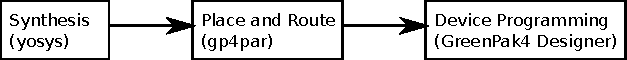
\includegraphics[scale=1]{figures/flow.pdf}
\caption{Data flow between toolchain components}
\label{flow}
\end{figure}

\subsection{Synthesis Example}

A simple synthesis script for \emph{yosys} is shown in figure \ref{yscript}. The script synthesizes a single Verilog 
source file \texttt{Blinky.v}, with a top-level module \texttt{BlinkyTop}, to the netlist \texttt{Blinky.json} and 
targets the SLG46620V. This script is only a starting point and may be customized as needed. This document does not
cover synthesis commands; please see the online documentation for \emph{yosys} for command documentation.
\begin{figure}[h]
\begin{lstlisting}[language=sh]
#!/usr/bin/env yosys
read_verilog Blinky.v
synth_greenpak4 -top BlinkyTop -part SLG46620V -json /tmp/Blinky.json
\end{lstlisting}
\caption{Example synthesis script}
\label{yscript}
\end{figure}

TODO: Include coding examples for inferring various hard IP? Or does this belong in the Yosys docs?

\pagebreak
\section{gp4par Limitations}

The following legal Verilog-2001 features are not supported by \emph{gp4par} as of this writing:

\begin{itemize}
\item {\bfseries Bidirectional or tri-state top-level module ports}\\All ports on top-level modules must be input or 
push-pull outputs. There is no support for tri-state or bidirectional outputs.
\item {\bfseries Non-scalar top-level module ports}\\All ports on top-level modules must be one bit wide. Vector ports 
may be used at lower levels of the hierarchy without restriction.
\end{itemize}

The following GreenPak4 device features are not supported by \emph{gp4par} as of this writing:

\begin{itemize}
\item All analog / mixed signal hard IP
\item All digital hard IP
\item Flipflops
\end{itemize}

\section{gp4par HDL Constraints}

There is only one supported constraint entry format at this time, Verilog attributes. There is currently no support for 
adding constraints to netlist entities via external constraint files or command line arguments. The general format of a 
constraint with name \texttt{FOO} and value 42 applied to the register \texttt{foobar} is shown in Figure 
\ref{constraint}.

\begin{figure}[h]
\begin{lstlisting}
(* FOO=42 *)
reg[3:0] foobar = 0;
\end{lstlisting}
\caption{Example Verilog attribute constraint}
\label{constraint}
\end{figure}

%%%%%%%%%%%%%%%%%%%%%%%%%%%%%%%%%%%%%%%%%%%%%%%%%%%%%%%%%%%%%%%%%%%%%%%%%%%%%%%%%%%%%%%%%%%%%%%%%%%%%%%%%%%%%%%%%%%%%%%%
% LOC

\pagebreak
\subsection{Physical Location (LOC)}

The LOC constraint instructs \emph{gp4par} to place the constrained net or primitive at a specific physical site of the 
device.

\subsubsection{Applicable Elements}
As of this writing, the LOC constraint may only be used on top-level module ports. 

\subsubsection{Constraint Values}
\begin{itemize}
\item {\bfseries Top-level module port}\\
Text string ``Pn" where \texttt{n} is the pin number of the device. Example: ``P3", ``P17".
\item {\bfseries Other} \\
This constraint may not be used on any other entity. Future versions of \emph{gp4par} may allow use of this constraint 
to lock LUTs, flipflops, and hard IP to specific locations.
\end{itemize}

\subsubsection{Verilog Usage Example}

Figure \ref{constraint-loc} is an example of a top-level module with three ports \texttt{a}, \texttt{b}, and \texttt{o}.
These ports are constrained to package pins 20, 19, and 18 respectively.

\begin{figure}[h]
\begin{lstlisting}
module Foo(a, b, o);

	(* LOC = "P20" *)
	input wire a;

	(* LOC = "P19" *)
	input wire b;

	(* LOC = "P18" *)
	output wire o;
	
endmodule
\end{lstlisting}
\caption{Example for LOC constraint}
\label{constraint-loc}
\end{figure}

%%%%%%%%%%%%%%%%%%%%%%%%%%%%%%%%%%%%%%%%%%%%%%%%%%%%%%%%%%%%%%%%%%%%%%%%%%%%%%%%%%%%%%%%%%%%%%%%%%%%%%%%%%%%%%%%%%%%%%%%
% Pulldown

\pagebreak
\subsection{Pull-Down Resistor (PULLDOWN)}

The PULLDOWN constraint instructs \emph{gp4par} to enable the pull-down resistor on the specified input. The exact resistor 
value ranges may be found in the device datasheet.

\subsubsection{Applicable Elements}
The PULLDOWN constraint may only be used on top-level module ports. 

\subsubsection{Constraint Values}
\begin{itemize}
\item {\bfseries Top-level module port (IOB)}\\
Text string ``10k", ``100k", or ``1M", case sensitive, to specify the nominal value of the pull-down resistor.
\item {\bfseries Other} \\
This constraint may not be used on any other entity.
\end{itemize}

\subsubsection{Verilog Usage Example}

Figure \ref{constraint-pulldown} is an example of a top-level module with three ports \texttt{a}, \texttt{b}, and
\texttt{o}. Ports \texttt{a} and \texttt{b} have 10k$\Omega$ pull-down resistors; port \texttt{o} is floating.

\begin{figure}[h]
\begin{lstlisting}
module Foo(a, b, o);

	(* PULLDOWN = "10k" *)
	input wire a;

	(* PULLDOWN = "10k" *)
	input wire b;

	input wire o;
	
endmodule
\end{lstlisting}
\caption{Example for PULLDOWN constraint}
\label{constraint-pulldown}
\end{figure}

%%%%%%%%%%%%%%%%%%%%%%%%%%%%%%%%%%%%%%%%%%%%%%%%%%%%%%%%%%%%%%%%%%%%%%%%%%%%%%%%%%%%%%%%%%%%%%%%%%%%%%%%%%%%%%%%%%%%%%%%
% Pullup

\pagebreak
\subsection{Pull-Up Resistor (PULLUP)}

The PULLUP constraint instructs \emph{gp4par} to enable the pull-up resistor on the specified input. The exact resistor 
value ranges may be found in the device datasheet.

\subsubsection{Applicable Elements}
The PULLUP constraint may only be used on top-level module ports. 

\subsubsection{Constraint Values}
\begin{itemize}
\item {\bfseries Top-level module port (IOB)}\\
Text string ``10k", ``100k", or ``1M", case sensitive, to specify the nominal value of the pull-up resistor.
\item {\bfseries Other} \\
This constraint may not be used on any other entity.
\end{itemize}

\subsubsection{Verilog Usage Example}

Figure \ref{constraint-pullup} is an example of a top-level module with three ports \texttt{a}, \texttt{b}, and
\texttt{o}. Ports \texttt{a} and \texttt{b} have 10k$\Omega$ pull-up resistors; port \texttt{o} is floating.

\begin{figure}[h]
\begin{lstlisting}
module Foo(a, b, o);

	(* PULLUP = "10k" *)
	input wire a;

	(* PULLUP = "10k" *)
	input wire b;

	input wire o;
	
endmodule
\end{lstlisting}
\caption{Example for PULLUP constraint}
\label{constraint-pullup}
\end{figure}

%%%%%%%%%%%%%%%%%%%%%%%%%%%%%%%%%%%%%%%%%%%%%%%%%%%%%%%%%%%%%%%%%%%%%%%%%%%%%%%%%%%%%%%%%%%%%%%%%%%%%%%%%%%%%%%%%%%%%%%%
% Schmitt Trigger

\pagebreak
\subsection{Schmitt Trigger (SCHMITT\_TRIGGER)}

The SCHMITT\_TRIGGER constraint instructs \emph{gp4par} to enable the Schmitt trigger on the specified input. The level 
of hysterisis provided may be found in the device datasheet.

\subsubsection{Applicable Elements}
The SCHMITT\_TRIGGER constraint may only be used on top-level module ports configured in bidirectional or input mode. 

\subsubsection{Constraint Values}
\begin{itemize}
\item {\bfseries Top-level module port (IOB)}\\
Any nonzero value, or no value, to enable the Schmitt trigger. Specify zero, or no constraint, to disable it.
\item {\bfseries Other} \\
This constraint may not be used on any other entity.
\end{itemize}

\subsubsection{Verilog Usage Example}

Figure \ref{constraint-schmitt} is an example of a top-level module with three ports \texttt{a}, \texttt{b}, and
\texttt{o}. The Schmitt trigger is enabled for ports  \texttt{a} and \texttt{b}, but not \texttt{o}.

\begin{figure}[h]
\begin{lstlisting}
module Foo(a, b, o);

	(* SCHMITT_TRIGGER = 1 *)
	input wire a;

	(* SCHMITT_TRIGGER *)
	input wire b;

	(* SCHMITT_TRIGGER = 0 *)
	input wire o;
	
endmodule
\end{lstlisting}
\caption{Example for SCHMITT\_TRIGGER constraint}
\label{constraint-schmitt}
\end{figure}

%%%%%%%%%%%%%%%%%%%%%%%%%%%%%%%%%%%%%%%%%%%%%%%%%%%%%%%%%%%%%%%%%%%%%%%%%%%%%%%%%%%%%%%%%%%%%%%%%%%%%%%%%%%%%%%%%%%%%%%%
% Timing constraints

\pagebreak
\section{gp4par Timing Constraints}

Static timing analysis is not yet implemented, thus this section is currently blank.

\pagebreak
\section{gp4par Verilog Primitives}

TODO: Document device-specific hard IP primitive wrappers here

\pagebreak
\section{gp4par Command Line Arguments}

\end{document}
